\documentclass[11pt]{article}
\usepackage[margin=1in]{geometry}
\usepackage[T1]{fontenc}
\usepackage{amsmath,amssymb,amsthm}
\usepackage{graphicx}
\usepackage[hidelinks]{hyperref}

\newtheorem*{theorem}{Literature-Implied Answer}

\title{A Literature-Implied Negative Answer to the Connes--Kirchberg Problem in arXiv:1101.4195}
\author{FA/Banach run packet}
\date{2026-06-14}

\begin{document}
\maketitle

\section*{Status}

This is a \texttt{literature\_implied\_answers} packet. It records that the
Connes--Kirchberg/QWEP problem stated in Pisier's survey
\cite{PisierSurvey} has a negative answer as a consequence of the later
\( \mathrm{MIP}^{*}=\mathrm{RE} \) theorem of
Ji--Natarajan--Vidick--Wright--Yuen \cite{MIPRE}, together with Kirchberg's
equivalence between the tensor-norm/QWEP formulation and Connes' embedding
problem as stated in the source paper. This is not an original proof from the
run.

\section*{Original Problem Evidence}

The relevant questions appear as Problems 12.9 and 12.10 on page 41 of the
downloaded source PDF. In the source TeX they are labelled
\texttt{prbl10.4} and \texttt{prbl10.4bis}.

\begin{center}

\includegraphics[width=\textwidth]{figures/open_problem_crop.png}
\end{center}

In words, the source asks whether, for \(A=C^*(\mathbb F_N)\), \(N>1\),
there is a unique \(C^*\)-norm on \(A\otimes A\), equivalently whether
\((A,A)\) is a nuclear pair. The adjacent formulation asks whether every
\(C^*\)-algebra is QWEP. The paragraph immediately above the problem states
that Kirchberg proved equivalence with Connes' embedding problem for finite
von Neumann algebras.

\section*{Supporting Answer Evidence}

The paper \( \mathrm{MIP}^{*}=\mathrm{RE} \) states in its abstract that,
using the known connection through Tsirelson's problem, the results refute
Connes' embedding conjecture.

\begin{center}
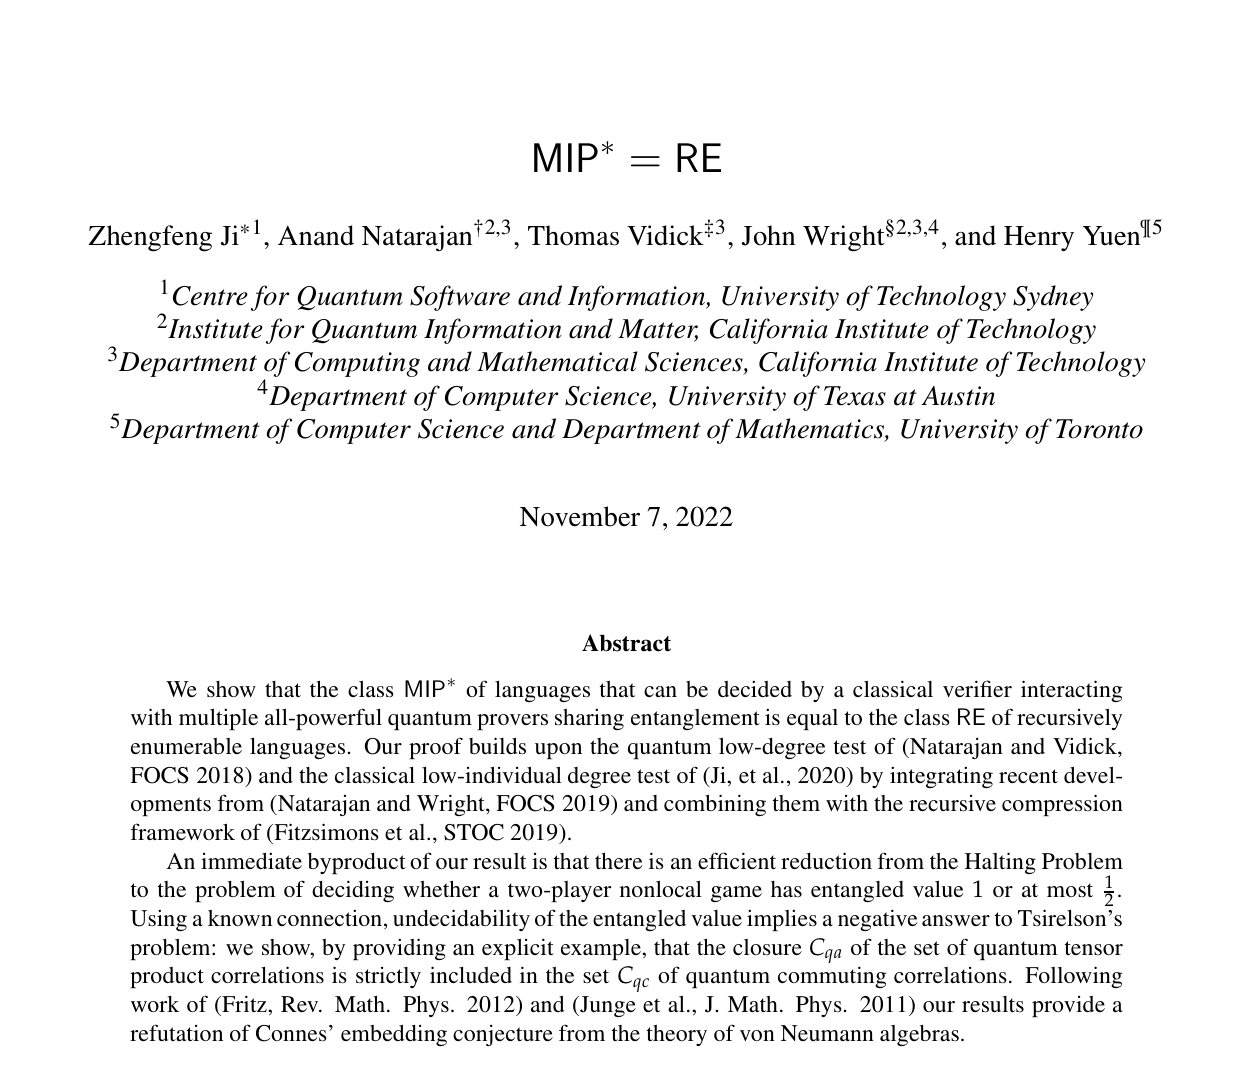
\includegraphics[width=\textwidth]{figures/mip_re_connes_refutation_crop.png}
\end{center}

Goldbring's later guided tour records the negative solution to CEP and
describes the traditional route through Kirchberg's QWEP problem.

\begin{center}
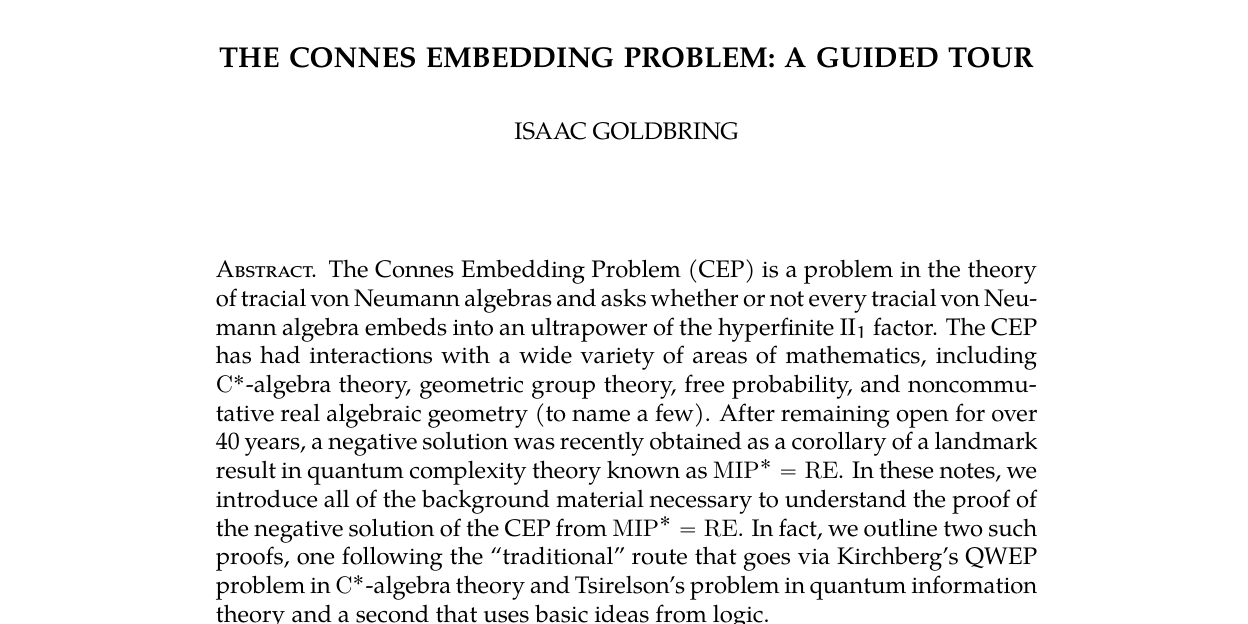
\includegraphics[width=\textwidth]{figures/goldbring_cep_qwep_negative_crop.png}
\end{center}

\section*{Idea of the Proof}

The source problem is an equivalent formulation of CEP: a positive answer to
the tensor-norm question for full group \(C^*\)-algebras of nonabelian free
groups is the same as a positive solution of the Kirchberg/QWEP/Connes
embedding problem. The later \( \mathrm{MIP}^{*}=\mathrm{RE} \) theorem
proves, through the quantum-correlation formulation, that CEP is false.
Transporting that negative result back through Kirchberg's equivalence gives
the negative answer to the tensor-norm and QWEP formulations in Pisier's
source paper.

\begin{theorem}
Problems 12.9 and 12.10 of \cite{PisierSurvey} have negative answers. In the
Kirchberg formulation, the full group \(C^*\)-algebra of a nonabelian free
group does not have a unique \(C^*\)-norm on its algebraic tensor square, and
not every \(C^*\)-algebra is QWEP.
\end{theorem}

\begin{proof}
Pisier's source states Problem 12.9 as the question whether, for
\(A=C^*(\mathbb F_N)\), \(N>1\), there is a unique \(C^*\)-norm on
\(A\otimes A\), equivalently whether \((A,A)\) is a nuclear pair. It then
states the equivalent QWEP formulation, Problem 12.10, asking whether every
\(C^*\)-algebra is QWEP. The surrounding discussion records Kirchberg's
equivalence between this problem and Connes' embedding problem.

Ji--Natarajan--Vidick--Wright--Yuen prove
\( \mathrm{MIP}^{*}=\mathrm{RE} \) and state that, following the known
connections through Tsirelson's problem, their result gives a refutation of
Connes' embedding conjecture \cite{MIPRE}. Goldbring's guided tour gives a
post-\(\mathrm{MIP}^{*}=\mathrm{RE}\) account of the same implication and
explicitly describes the traditional route through Kirchberg's QWEP problem
\cite{GoldbringGuide}.

Therefore Connes' embedding problem is false. Since Pisier's tensor-norm and
QWEP questions are equivalent to it, those questions are false as well. Thus
the algebraic tensor product \(C^*(\mathbb F_N)\otimes C^*(\mathbb F_N)\) in
Kirchberg's nonabelian free-group formulation cannot have a unique
\(C^*\)-norm, and there must exist \(C^*\)-algebras that are not QWEP.
\end{proof}

\section*{Limitations}

This packet addresses only the Connes--Kirchberg/QWEP problem cluster in
Pisier's survey. The survey contains many other open problems, including
questions about exact Grothendieck constants, noncommutative Khintchine
inequalities, and multilinear operator-space Grothendieck-type problems.
Those are not claimed here.

\section*{Verification Notes}

The source and supporting papers are distinct. The route is an implication
through Kirchberg's equivalence, so the packet belongs in the
literature-implied bucket rather than the already-answered bucket. The local
duplicate search covered the arXiv ids 1101.4195, 2001.04383, and
2109.12682, together with the phrases Connes Embedding, QWEP, Kirchberg, and
MIP*. No existing packet or attempt covered this exact status identification.
No computation is involved.

\section*{Human Review Recommendation}

Check three points: first, that Pisier's Problem 12.9/12.10 is indeed the
Kirchberg/QWEP formulation equivalent to CEP; second, that \cite{MIPRE}
establishes the negative CEP consequence; and third, that the nonabelian
free-group tensor-norm formulation in the source is covered by the standard
Kirchberg equivalence. If these are accepted, the negative answer follows.

\begin{thebibliography}{9}

\bibitem{PisierSurvey}
G. Pisier,
\emph{Grothendieck's theorem, past and present},
Bull. Amer. Math. Soc. 49 (2012), no. 2, 237--323;
arXiv:1101.4195.

\bibitem{MIPRE}
Z. Ji, A. Natarajan, T. Vidick, J. Wright, and H. Yuen,
\emph{\( \mathrm{MIP}^{*}=\mathrm{RE} \)},
Commun. ACM 64 (2021), no. 11, 131--138;
arXiv:2001.04383.

\bibitem{GoldbringGuide}
I. Goldbring,
\emph{The Connes Embedding Problem: A guided tour},
arXiv:2109.12682.

\end{thebibliography}

\end{document}
